\chapter{پیاده‌سازی و نتایج نو}

در این پروژه، (تا جایی که نویسنده اطلاع دارد) برای اولین بار از الگوریتم‌های یادگیری ماشین کوانتومی برای تولید موسیقی استفاده شده است. همان‌طور که در بخش
\ref{sec:parts}
اشاره شد، این پروژه شامل سه ماژول 
\lr{Midi}،
\lr{QLSTM}
و
\lr{QuGAN}
است که در این فصل توضیحات کامل عملکرد آن‌ها شرح داده می‌شود.
شایان ذکر است که موسیقی‌های تولید شده توسط این مدل، دارای تندای\fnote{Tempo} ثابت هستند؛ به این معنا که فاصله‌ی بین نت‌های مختلف همیشه یکسان و برابر با پنجاه میلی‌ثانیه است.
عملیات‌های مربوط به تئوری موسیقی، پردازش مجموعه داده به عنوان ورودی پروژه و تولید فایل‌های موسیقی به عنوان خروجی پروژه با استفاده از کتابخانه‌ی
\lr{Music21}
صورت می‌گیرد.
مدارهای کوانتومی این پروژه، با استفاده از کتابخانه‌ی 
\lr{PennyLane}
که کتابخانه‌ای مختص یادگیری ماشین کوانتومی است طراحی شده‌اند و بهینه‌سازی پارامترهای این مدارها، با استفاده از رابط کاربری بین این کتابخانه و کتابخانه‌ی
\lr{PyTorch}
انجام شده است.
لازم به ذکر است که در این پروژه، به علت در دسترس نبودن کامپیوترهای کوانتومی موردنیاز، محاسبات کوانتومی توسط شبیه‌سازی کوانتومی موجود در کتابخانه‌ی
\lr{PennyLane}
انجام می‌گیرد.

\begin{figure}
	\centering
	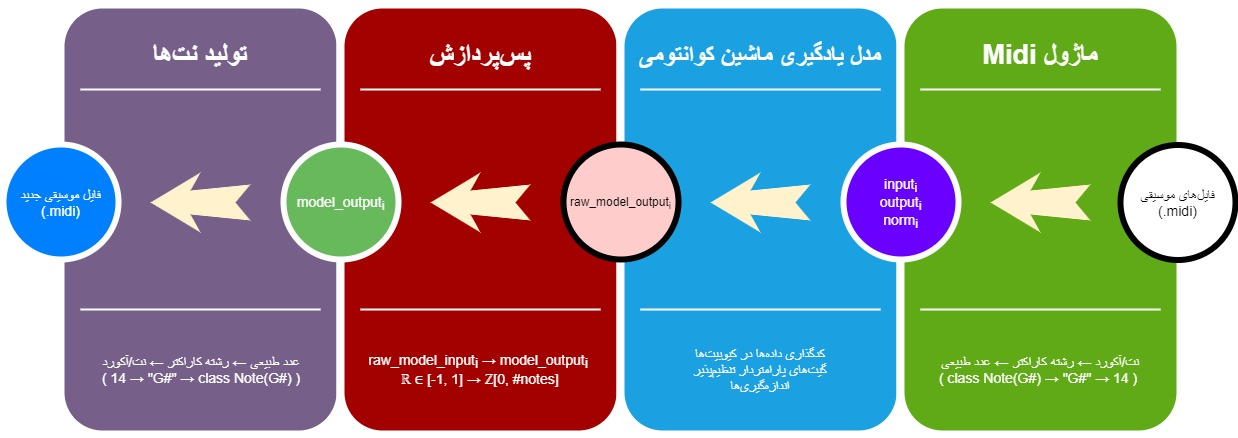
\includegraphics[scale=0.355]{figures/Diagram.jpg}
	\caption{دیاگرام مراحل کلی پیاده‌سازی شده در پروژه}
	\label{fig:diagram}
\end{figure}

\section{مراحل کلی پروژه}
مراحل کلی پیاده‌سازی شده در این پروژه، در شکل
\ref{fig:diagram}
آمده است.
توضیح این شکل به طور خلاصه به این صورت است: در مرحله‌ی اول، مجموعه داده‌ی این پروژه که به صورت تعدادی فایل موسیقی شامل نت‌ها و آکوردها با پسوند
\lr{midi}
است، به عنوان ورودی وارد ماژول
\lr{Midi}
می‌شود. این ماژول در ابتدا نگاشتی از نت‌ها و آکوردهای فایل‌های ورودی به اعداد طبیعی می‌سازد، سپس مجموعه‌ای از جفت ورودی و خروجی‌ها به صورت اعداد طبیعی را تولید می‌کند. در مرحله‌ی دوم، مجموعه‌ی تولید شده به عنوان ورودی وارد یک مدل یادگیری ماشین کوانتومی (که یکی از ماژول‌های 
\lr{QLSTM} 
یا
\lr{QuGAN}
است) می‌شود. در مرحله‌ی سوم، خروجی‌های تولید شده توسط مدل یادگیری ماشین کوانتومی که اعدادی حقیقی در بازه‌ی
$[-1, 1]$
هستند، وارد مرحله‌ی پس‌پردازش می‌شوند تا این اعداد، به اعدادی طبیعی تبدیل شوند.
در نهایت، خروجی‌های مرحله‌ی پس‌پردازش به تابعی به نام
$generate\_notes$
داده می‌شود تا از روی این اعداد طبیعی، نت‌ها و آکوردهای جدیدی ساخته شوند و در یک فایل با پسوند
\lr{midi}
ذخیره شوند. این فایل حاوی موسیقی جدید تولید شده توسط پروژه است.

\section{ماژول 
\lr{Midi}
} \label{sec:midi_module}
ماژول
\lr{Midi}
مسئولیت پیش‌پردازش داده‌ها برای استفاده از مدل‌های یادگیری ماشین کوانتومی را بر عهده دارد.
مجموعه داده‌ی این پروژه، شامل ۹۲ قطعه‌ی موسیقی پیانو به صورت فایل‌های 
\lr{midi}
است، هرکدام از این فایل‌ها، مجموعه‌ای از نت‌ها، آکوردها و زمان پخش آن نت/آکورد از ابتدای قطعه به میلی‌ثانیه است.
این ماژول، با استفاده از کتاب‌خانه‌ی 
\lr{Music21}
تنها یک‌بار پوشه‌ی شامل مجموعه داده‌ها را به صورت کامل بررسی کرده، نت‌های تمامی قطعات را به صورت متوالی در یک لیست ذخیره کرده و در نهایت در یک فایل واحد با نام
\lr{notes.pk}
ذخیره می‌کند. شایان ذکر است که در صورت برخورد با یک آکورد، نت‌های آن را استخراج کرده و همانند چند نت عادی که پشت سر هم پخش می‌شوند، آن‌ها را به لیست نت‌ها اضافه می‌کند.
در عین حال، برای قابل‌فهم کردن نت‌ها برای یک مدل یادگیری ماشین، یک نگاشت ۱-به-۱
از نت‌ها به اعداد طبیعی ساخته می‌شود.
این ماژول سپس در هر بار اجرای کد، با گرفتن پارامتری به نام
\lr{SequenceLength}
تعداد زیادی جفت ورودی و خروجی برای مدل یادگیری ماشین کوانتومی فراهم می‌کند؛ به این صورت:

\begin{equation}
    \begin{gathered}
    input_i = [inotes_{(i)}, ..., inotes_{(SequenceLength + i)}] \\[3pt]
    norm_i = \sqrt{\sum^{SequenceLength+i}_{k=i} (inotes_{(k)})^2 } \\[3pt]
    output_i = [inotes_{(SequenceLength + i + 1)}] \\[3pt]
    where \hso 0 \leq i \leq n - SequenceLength - 1 \hso ; \hso n = \#notes
    \end{gathered}
\end{equation}
\myequations{نحوه تولید ورودی و خروجی ماژول \lr{Midi}}
که در معادله‌ی بالا،
$inotes_{(i)}$
برابر با عدد طبیعی‌ای‌ست که معادل
$i$-
امین نت در مجموعه نت‌هاست.


\section{ماژول
\lr{QLSTM}
} \label{sec:qlstm_module}
هدف این ماژول، تولید موسیقی با استفاده از حافظه‌های طولانی کوتاه مدت کوانتومی است. در این بخش، جزئیات پیاده‌سازی این ماژول شرح داده می‌شوند.
در کتابخانه‌ی 
\lr{PyTorch}،
هر مدل آموزش‌پذیر یادگیری ماشین، زیرکلاسی از کلاس 
\lr{torch.nn.Module}
است. به همین دلیل، کلاس‌های این ماژول، همگی زیرکلاسی از
\lr{torch.nn.Module}
هستند.
یکی از توابع مهم کلاس
\lr{torch.nn.Module}،
تابع
\lr{forward}
است که در هر بار اجرا، مقداری داده به عنوان ورودی گرفته و با اعمال یک الگوریتم یادگیری ماشین به این ورودی‌ها، نتایج تولید شده توسط این الگوریتم را به عنوان خروجی می‌دهد.
این کلاس‌ها در زیر شرح داده می‌شوند.

\subsection{طراحی اولیه}
طراحی اولیه‌ی این ماژول، الهام گرفته از پیاده‌سازی‌های معمول تولید موسیقی با استفاده از حافظه‌های طولانی کوتاه مدت کلاسیک بود که در بخش زیر به این پیاده‌سازی‌های کلاسیک پرداخته می‌شود:
\subsubsection{پیاده‌سازی کلاسیک}
ایده‌ی کلی این پیاده‌سازی‌ها به این صورت است که در اولین مرحله،
$output_i$
های تولید شده در ماژول 
\lr{Midi}،
با استفاده از کدگذاری یک بارز\fnote{One-hot encoding} شکل جدیدی پیدا می‌کنند. این کدگذاری به این صورت انجام می‌شود که اگر 
\lr{n}
تعداد
$output_i$
وجود داشته باشد، داده‌ی
\lr{k}
ام این مجموعه که
$output_k$
نام دارد، تبدیل به برداری
\lr{n}
بعدی می‌شود که همه‌ی ورودی‌های آن صفر است و تنها 
\lr{k}
امین ورودی آن برابر با یک قرار می‌گیرد.
در این مساله، عدد 
\lr{n}
برابر با تعداد نت‌های منحصر به فرد موجود در لیست
\lr{notes}
تولید شده در ماژول
\lr{Midi}
در نظر گرفته می‌شود.
سپس، با گرفتن ابعاد بردارهای ورودی و خروجی گیت‌های بازگشتی به عنوان ورودی، ابعاد ماتریس‌های
\lr{W} و \lr{U}
که در معادله‌ی
\ref{eqn:lstm_gate}
تعریف شده بودند تعیین می‌شود و واحدهای بازگشتی با استفاده از این ابعاد و پارامتر حذفی که برابر با ۳.۰ است ساخته می‌شوند. پس از قرار دادن تعدادی لایه‌ی بازگشتی پشت سر هم، ابتدا خروجی‌های لایه‌های مختلف تحت تاثیر یک لایه‌ی خطی که در کتابخانه‌ی
\lr{PyTorch}
به صورت کلاس
\lr{torch.nn.Linear}
پیاده‌سازی شده است قرار می‌گیرند. کارکرد این لایه به این صورت است که با گرفتن سه عدد
$n, m$ و $b$
برداری 
$n$
بعدی را با استفاده از تبدیل خطی زیر، تبدیل به برداری
$m$
بعدی می‌کند:
% \vspace{-1mm}
\begin{equation}
\begin{gathered}
       y = Ax + b \\
       dim(A) = m * n
\end{gathered}
\end{equation}
\myequations{نحوه‌ی کارکرد کلاس \lr{torch.nn.Linear}}
% \vspace{-3mm}
دلیل وجود این لایه‌ی خطی این است که بردارهایی که توسط خروجی‌های واحدهای بازگشتی ساخته شده، تبدیل به بردارهایی با طول
\lr{n}
شوند.  این کار باعث می‌شود خروجی‌های مدل، با خروجی‌هایی که تحت کدگذاری یک بارز قرار گرفته بودند، قابل مقایسه شوند.
در انتها، بردار نهایی تولید شده به عنوان برداری از احتمالات خروجی داده شدن هر کدام از نت‌های موجود در لیست 
\lr{notes}
تعبیر می‌شود و تابع آنتروپی متقاطع
\fnote{Cross Entropy}
به عنوان تابع هزینه‌ی این مدل در نظر گرفته می‌شود.
تابع آنتروپی متقاطع به این صورت تعریف می‌شود که اگر
\lr{N}
عدد دسته‌بندی وجود داشته باشد و برداری 
\lr{N}
بعدی به نام 
\lr{x}
به عنوان ورودی به این تابع داده شود، خروجی آن به صورت معادله‌ی زیر خواهد بود:

\begin{equation}
    \begin{gathered}
       loss(x, class) = -log\big(\frac{exp(x[class])}{\sum_j exp(x[j])}\big) = -x[class] + log\big(\sum_j exp(x[j])\big) \\
       loss = \frac{
        \sum_{i=1}^{N} loss(i, class[i])
       }{N}
    \end{gathered}
\end{equation}
\myequations{تابع آنتروپی متقاطع}

در مراحل اولیه‌ی پروژه، این پیاده‌سازی کلاسیک به کمک کتابخانه‌ی
\lr{PyTorch}
به طور کامل انجام شد تا از انجام‌پذیر بودن کلیت مساله اطمینان حاصل شود.

\subsubsection{پیاده‌سازی کوانتومی}
در مرحله‌ی بعد، سعی شد تا با جایگزین کردن حافظه‌ی طولانی کوتاه مدت کلاسیک با یک حافظه‌ی طولانی کوتاه مدت کوانتومی، الگوریتمی کوانتومی برای تولید موسیقی طراحی شود. حافظه‌ی طولانی کوتاه مدت  کوانتومی استفاده شده در این بخش، بر اساس مدلی که در بخش
\ref{sec:qlstm}
معرفی شد طراحی شده است.
بعد از پیاده‌سازی و انجام تست‌های مختلف بر روی این پیاده‌سازی با استفاده از ابرپارامترهای متفاوت، به این نتیجه رسیده شد که این‌گونه پیاده‌سازی، تنها می‌تواند با یادگیری بر روی هر مجموعه داده، یک نت ثابت تولید کند. این مساله به این دلیل است که اختلاف بسیار زیادی بین تعداد نت‌های منحصر به فرد موجود در مجموعه داده و تعداد کیوبیت‌های قابل شبیه‌سازی بر روی کامپیوترهای کلاسیک وجود دارد؛ این امر باعث می‌شود که پارامترهای موجود در لایه‌ی
\lr{torch.nn.Linear}
مدل، نتوانند به تبدیل مناسبی از برداری با بعد پایین که از خروجی اندازه‌گیری‌های کیوبیت‌ها تولید شده است به برداری با بعدی به اندازه‌ی تعداد نت‌های منحصر به فرد موجود در مجموعه داده دست پیدا کنند. به همین خاطر، در نسخه‌ی کنونی پروژه معماری متفاوتی برای استفاده از حافظه‌های طولانی کوتاه مدت کوانتومی پیشنهاد شده که جزئیات آن به صورت کامل در بخش‌های بعدی بیان شده است.

% بخش کوانتومی ماژول
% \lr{QLSTM}
% بر اساس حافظه‌های طولانی کوتاه-مدت کوانتومی که در بخش
% \ref{sec:qlstm}
% معرفی شدند طراحی شده است.
% \newparagraph

\begin{figure}
    \centering
    \begin{quantikz}
            \lstick[wires=3]{$\ket{0}^{\otimes n\_qubits}$} & \gate[wires=3][2cm]{AE(x)} & \gate[wires=3][2cm]{RL_1(\theta_1)} &\qw &\ldots &\ & \gate[wires=3][2cm]{RL_k(\theta)} & \qw & \meter{}  \\
            & \qw & \qw & \qw & \ldots & & \qw & \qw & \meter{} \\
            & \qw & \qw & \qw & \ldots & & \qw & \qw & \meter{}
    \end{quantikz}
    \caption{نمایش دیداری مدار کوانتومی استفاده شده در حافظه‌ی طولانی کوتاه مدت کوانتومی}
    \label{fig:qrecursive}
\end{figure}

\newpage
\subsection{
کلاس
\lr{QLSTMCell}
}

\begin{algorithm}[t]
\caption{نحوه‌ی کارکرد یک واحد بازگشتی در حافظه‌ی طولانی کوتاه مدت کوانتومی} \label{alg:qlstmcell}
\lr{
    \begin{algorithmic}
        \STATE $c_{t-1}$ \hso $\leftarrow$ Cell state vector from the previous cell
        \STATE $h_{t-1}$ \hso $\leftarrow$ Hidden state vector from the previous cell
        \STATE $x_{t}$ \hso $\leftarrow$ Current cell's input
        \STATE drop \hso $\leftarrow$ Current cell's dropout value
        \STATE VQC\_forget \hso $\leftarrow$ pre-generated quantum recurrent gate
        \STATE VQC\_input \hso $\leftarrow$ pre-generated quantum recurrent gate
        \STATE VQC\_update \hso $\leftarrow$ pre-generated quantum recurrent gate
        \STATE VQC\_output \hso $\leftarrow$ pre-generated quantum recurrent gate
        \STATE $y_{t} = [h_{t-1} \hso ; \hso x]$
        \STATE $f_{t} = sigmoid(VQC\_forget(y_{t}))$
        \STATE $i_{t} = sigmoid(VQC\_input(y_{t}))$
        \STATE $g_{t} = sigmoid(VQC\_update(y_{t}))$
        \STATE $o_{t} = sigmoid(VQC\_output(y_{t}))$
        \STATE $c_{t} = (f_{t} * c_{t}) + (i_{t} * g_{t})$
        \STATE $h_{t} = o_{t} * tanh(c_{t})$
        \STATE $h_{t} = dropout(h_{t}, drop)$
    \end{algorithmic} 
}
\end{algorithm}
\myalgorithms{
   نحوه‌ی کارکرد یک واحد بازگشتی در حافظه‌ی طولانی کوتاه مدت کوانتومی
}

هر واحد بازگشتی کوانتومی این الگوریتم در کلاس
\lr{QLSTMCell}
تعریف شده.
ورودی‌های مهمی که برای ساختن نمونه‌ای از این کلاس لازم است به شرح زیر هستند:
\begin{itemize}
    \item 
    \lr{n\_qubits}
    تعداد کیوبیت‌های استفاده شده در مدارهای کوانتومی این واحد بازگشتی است.
    \item
    \lr{n\_qlayers}
    تعداد لایه‌های موجود در قسمت پارامتردار مدارهای کوانتومی را تعیین می‌کند.
    \item
    \lr{hidden\_size}
    ابعاد داده‌های ورودی و خروجی واحد بازگشتی را تعیین می‌کند.
\end{itemize}

این کلاس سپس با استفاده از پارامترهای دریافت شده، چهار مدار کوانتومی برای گیت‌های بازگشتی می‌سازد.
هر کدام از این مدارهای کوانتومی، از ترکیب تابع کدگذاری
\lr{AmplitudeEmbedding}
و تابع پارامتریک
\lr{RandomLayers}
کتابخانه‌ی
\lr{PennyLane}
ساخته شده است.

هر تابع
\lr{AmplitudeEmbedding}
با دریافت ورودی‌ای با ابعاد
$2^n$،
آن را در 
$n$
کیوبیت هدف به صورت زیر کدگذاری می‌کند:
\begin{equation} \label{eqn:midi_data}
    \begin{gathered}
       input = [x_0, x_1, \dots, x_{2^n-1}] \hst ; \hst x_i \in \mathbb{R} \\[3pt]
       norm = \sqrt{\sum^{2^n}_{i=0} x_i^2 } \\[3pt]
       output = \frac{x_0}{norm} |00...0\rangle + \frac{x_1}{norm} |00...1\rangle + ... + \frac{x_{2^n-1}}{norm} |11...1\rangle
    \end{gathered}
\end{equation}
\myequations{
نحوه‌ی کارکرد تابع
\lr{AmplitudeEmbedding}
}

و هر تابع 
\lr{RandomLayers}
با دریافت یک ورودی با ابعاد
$(L, k)$
و یک عدد طبیعی
\lr{seed}
،تعداد
$L$
لایه‌ی پارامتریک را با استفاده از
\lr{seed}
به صورت تصادفی تولید می‌کند.
هر لایه‌ی تولید شده توسط
\lr{RandomLayers}
شامل ترکیبی از 
$k$
گیت کوانتومی پارامتریک و تعدادی گیت 
$CNOT$
است.


نمایش دیداری این گیت‌های بازگشتی کوانتومی، در شکل
\ref{fig:qrecursive}
آمده است که این شکل، دقیقا حالت خاصی از شکل
\ref{fig:qml_visualization}
است که در آن، از 
\lr{AmplitudeEmbedding}
برای لایه‌ی کدگذاری و از
\lr{RandomLayers}
برای لایه‌ی پارامتریک استفاده شده است.
لازم به ذکر است که در این شکل به جهت اختصار از عبارت
\lr{AE}
به جای
\lr{AmplitudeEmbedding}
و از عبارت
\lr{RL}
به جای 
\lr{RandomLayers}
استفاده شده است.

پس هر واحد بازگشتی در پیاده‌سازی فعلی، یک
\lr{QLSTMCell}
است که مدارهای کوانتومی آن، از پشت سر هم قرار گرفتن زیرمدارهای تولید شده توسط
\lr{AmplitudeEmbedding}
و
\lr{RandomLayers}
ساخته شده‌اند و در نهایت، آرایه‌ای متشکل از امیدریاضی اندازه‌گیری جداگانه‌ی تک‌تک کیوبیت‌های هر مدار به عنوان خروجی آن مدار در نظر گرفته می‌شود.
فرم شبه‌کدی الگوریتم اجرا شده در هر بار اجرای تابع
\lr{forward}
یک کلاس
\lr{QLSTMCell}
به صورت کامل در الگوریتم
\ref{alg:qlstmcell}
آمده است. در این الگوریتم، متغیرهای
$c_{t-1}$ و
$h_{t-1}$
که به ترتیب بردار وضعیت واحد و بردار وضعیت پنهان واحد بازگشتی قبلی هستند به صورت ورودی داده می‌شوند. متغیر
$x_{t}$
نیز که ورودی واحد بازگشتی کنونی است، از مجموعه داده‌ی پروژه به صورت ورودی به این الگوریتم داده می‌شود. هم‌چنین، توابع
\lr{VQC\_forget}،
\lr{VQC\_input}،
\lr{VQC\_update} و
\lr{VQC\_output}
مدارهای کوانتومی‌ای هستند که از پیش با استفاده از پارامترهای
\lr{n\_qubits}
و
\lr{n\_qlayers}
ساخته شده‌اند و ساختارشان به صورتی که در شکل
\ref{fig:qrecursive}
ترسیم شده قرار دارد.
\lr{drop}
که پارامتر حذف این واحد بازگشتی است نیز به عنوان ورودی به این الگوریتم داده می‌شود.

\begin{algorithm}[t]
\caption{نحوه‌ی کارکرد یک حافظه‌ی طولانی کوتاه مدت کوانتومی} \label{alg:full_qlstm}
\lr{
    \begin{algorithmic}
        \STATE n\_layers \hso $\leftarrow$ Number of QLSTMCell's present in this QLSTM
        \STATE QLSTMCells \hso $\leftarrow$ A list of initialized QLSTMCell's
        \STATE inputs \hso $\leftarrow$ A list of inputs generated by the Midi module
        \STATE outputs \hso $\leftarrow$ Empty list
        \STATE $h_{t} = [0, \dots, 0]$
        \STATE $c_{t} = [0, \dots, 0]$
        \FOR {$ i=0 \to$ n\_layers}
            \STATE $h_{t}, c_{t} = QLSTMCells[i](inputs[i], h_{t}, c_{t})$
            \STATE outputs.add$(c_{t})$
        \ENDFOR
    \end{algorithmic} 
}
\end{algorithm}
\myalgorithms{
   نحوه‌ی کارکرد یک حافظه‌ی طولانی کوتاه مدت کوانتومی
}

\subsection{
کلاس
\lr{QLSTM}
}

این کلاس با دریافت ورودی‌ای با نام
\lr{n\_layers}،
تعداد
\lr{n\_layers}
لایه از 
\lr{QLSTMCell}
ها را در کنار هم قرار می‌دهد و تغییرات لازم برای رد کردن خروجی‌های هرکدام از این لایه‌ها به عنوان ورودی لایه‌ی بعدی را انجام می‌دهد. این کلاس در هر بار اجرا، آرایه‌ای به نام
\lr{outputs}
که مجموعه‌ی خروجی‌های تولید شده توسط 
\lr{n}
لایه از واحدهای بازگشتی کوانتومی است را خروجی می‌دهد.
فرم شبه‌کدی الگوریتم اجرا شده در هر بار اجرای تابع
\lr{forward}
کلاس 
\lr{QLSTM}
به صورت کامل در الگوریتم
\ref{alg:full_qlstm}
آمده است.

\subsection{
کلاس
\lr{QLSTMusic}
}
این کلاس با گرفتن ورودی و خروجی‌های تولید شده از ماژول
\lr{Midi}
و یک عدد طبیعی به نام
\lr{n\_epochs}،
به تعداد
\lr{n\_epochs}
بار
ورودی و خروجی‌ها را به یک 
\lr{QLSTM}
رد می‌کند و بعد از انجام پس‌پردازش روی خروجی‌های تولید شده، پارامترهای آن را برای کمینه‌کردن یک تابع هزینه بهینه‌سازی می‌کند. چگونگی انجام این پس‌پردازش به طور کامل در بخش بعد شرح داده شده است.

\subsection{پس‌پردازش} \label{sec:qlstm_post}
\begin{algorithm}[t]
\caption{پس‌پردازش ماژول \lr{QLSTM}}  \label{alg:qlstmpost}
\lr{
    \begin{algorithmic}
        \STATE $raw\_model\_output_i = QLSTMCells[i](input_i)$
        \STATE $model\_output_i = mean(raw\_model\_output_i)$
        \STATE $model\_output_i = model\_output_i * norm_i$
    \end{algorithmic}
}
\end{algorithm}
\myalgorithms{
    پس‌پردازش ماژول
    \lr{QLSTM}
}
هر لایه از
\lr{QLSTM}
که شامل
$n$
کیوبیت باشد، 
$n$
خروجی که هر کدام از آن‌ها عددی در بازه‌ی
$[-1, 1]$
است تولید می‌کند. به همین دلیل، برای تبدیل کردن این اعداد به اعداد طبیعی‌ای که معادل نت‌های مجموعه داده باشند، باید روی خروجی‌ها پس‌پردازش انجام داد.
پس‌پردازش پیشنهادی در این مرحله، در الگوریتم
\ref{alg:qlstmpost}
آمده است. در این الگوریتم، متغیرهای
$input_i$
و
$norm_i$
طبق معادله‌ی
\ref{eqn:midi_data}
تعریف شده‌اند،
$raw\_model\_output_i$
خروجی اولیه‌ای است که از مدار کوانتومی گرفته می‌شود و
$model\_output_i$
خروجی نهایی بعد از پس‌پردازش است.



% برای هر
% \lr{QLSTMCell}،
% پس از پاس‌داده‌شدن
% $input_i$
% به شکلی که در معادله‌ی
% \ref{eqn:midi_data}
% تعریف شده، 
% یک
% $modelOutput_i$
% تولید می‌شود که شامل
% $n$
% عدد است.
% ابتدا از خروجی‌های داده‌شده توسط هر کدام از واحدهای بازگشتی میانگین گرفته می‌شود و سپس با ضرب این میانگین
% در
% $norm_i$،
% عدد طبیعی معادل نت پیشنهادی هر
% \lr{QLSTMCell}
% تولید می‌شود.

\subsection{تابع هزینه}
به علت این‌که ممکن است عدد طبیعی معادل نت پیشنهادی، بزرگ‌تر یا کوچک‌تر از عدد طبیعی معادل نت خروجی مجموعه داده باشد، از تابع خطای میانگین مربعات که در معادله‌ی
\ref{eqn:mse}
معرفی شد، به عنوان تابع هزینه استفاده می‌شود.
علت مناسب بودن این تابع هزینه، این است که در هنگام ساخت نگاشت یک به یک از نت‌ها به اعداد طبیعی، مرتب‌سازی به گونه‌ای انجام شد که هرچه‌قدر فرکانس نت‌ها به هم نزدیک‌تر باشد، اعداد طبیعی متناظر آن‌ها نیز به هم نزدیک‌تر باشند.

در نهایت، تابع
\lr{generate\_notes}
با گرفتن پارامتر
\lr{n\_notes}
با چندین‌بار اجرای الگوریتم‌های یادگیری ماشین و پس‌پردازش، به تعداد
\lr{n\_notes}
نت موسیقی جدید تولید کرده و با قرار دادن فاصله‌هایی به اندازه‌ی پنجاه میلی‌ثانیه بین آن‌ها، نتایج حاصل را در یک فایل با پسوند
\lr{midi}
ذخیره می‌کند.


\section{
ماژول
\lr{QuGAN}
}
ماژول
\lr{QuGAN}
بر اساس شبکه‌های زایای دشمن‌گونه‌ی کوانتومی که در بخش
\ref{sec:qugan}
معرفی شد طراحی شده است.
این ماژول نیز همانند ماژول
\lr{QLSTM}
از ماژول
\lr{Midi}
برای پیش‌پردازش داده‌ها استفاده می‌کند.

این ماژول به طور کلی شامل سه زیرمدار کوانتومی است. از ترکیب‌های مختلف این سه زیرمدار، سه مدار کوانتومی تشکیل می‌شود که توضیح کارکرد آن‌ها در زیر آمده است:

\begin{itemize}
    \item زیرمدار اول که در کد پروژه توسط تابع
    \lr{encode\_music}
    ساخته می‌شود، با دریافت نت‌هایی به عنوان ورودی، آن‌ها را با استفاده از تابع
    \lr{AmplitudeEmbedding}
    در کیوبیت‌های سیستم کدگذاری می‌کند.
    
    \item زیرمدار دوم که زیرمداری پارامتریک است و در کد پروژه توسط تابع
    \lr{discriminator}
    ساخته می‌شود، با استفاده از تابع
    \lr{RandomLayers}
    لایه‌هایی پارامتریک تولید می‌کند. این لایه‌ها سعی در تشخیص واقعی یا ساختگی بودن داده‌های موجود در کیوبیت‌ها دارند و عمل‌کرد متمایزکنندگی شبکه را پیاده‌سازی می‌کنند.
    خروجی این زیرمدار، آرایه‌ای متشکل از امیدریاضی اندازه‌گیری تک‌تک کیوبیت‌های سیستم به صورت مجزا است.
    
    \item زیرمدار سوم، همانند زیر مدار دوم مداری پارامتریک است، اما سعی در تولید داده‌هایی ساختگی از روی کیوبیت‌هایی که مقداری نویز به عنوان داده‌ی اولیه بر روی آن‌ها کدگذاری شده‌اند دارد. این زیرمدار در کد پروژه توسط تابع
    \lr{music\_generator}
    ساخته می‌شود و عملکرد زایایی شبکه را پیاده‌سازی می‌کند.
\end{itemize}

و مدارهای کوانتومی این ماژول، به این شکل ساخته شده‌اند:
\begin{itemize}
    \item
    مدار اول که
    \lr{real\_music\_discriminator}
    نام دارد،
    ابتدا به کمک تابع
    \lr{encode\_music}
    تعدادی نت از مجموعه داده گرفته و آن‌ها را در کیوبیت‌های سیستم کدگذاری می‌کند، سپس زیرمدار
    \lr{discriminator}
    سعی می‌کند با بهینه‌سازی پارامترهای خود تشخیص دهد آیا داده‌ها واقعی هستند یا خیر.
    
    \item
    مدار دوم که
    \lr{generated\_music\_discriminator}،
    نام دارد، ابتدا با گرفتن مقداری نویز به عنوان ورودی، آن نویزها را توسط
    \lr{encode\_music}
    در سیستم کدگذاری می‌کند، سپس زیرمدار \\
    \lr{music\_generator}
    با بهینه‌سازی پارامترهای خود، اقدام به ساخت داده‌ی جدیدی از روی نویز کدگذاری شده می‌کند و در نهایت، زیرمدار
    \lr{discriminator}
    سعی می‌کند با بهینه‌سازی پارامترهای خود، تشخیص دهد آیا داده یکی از داده‌های واقعی است یا خیر.
    
    \item
    مدار سوم که
    \lr{final\_music\_generator}
    نام دارد، با ترکیب زیرمدار‌های
    \lr{encode\_music}
    و \\
    \lr{music\_generator}
    ابتدا مقداری نویز را در سیستم کدگذاری کرده و سپس آرایه‌ای متشکل از امیدریاضی اندازه‌گیری تک‌تک کیوبیت‌های سیستم را به عنوان خروجی تولید می‌کند که نتیجه‌ی نهایی الگوریتم، از این خروجی ساخته می‌شود.
    
\end{itemize}
نکته‌ی اصلی این است که بعد از هربار اجرای مدارهای اول و دوم، وزن‌های زیرمدار
\lr{discriminator}
آن‌ها با هم همگام می‌شوند، چراکه در کل برنامه باید تنها یک
\lr{discriminator}
وجود داشته‌باشد.

بعد از ساخته‌شدن این مدارها، با استفاده از توابع هزینه‌ی معرفی شده در معادله‌ی
\ref{eqn:qugan_cost}
پارامترهای زیرمدارهای 
\lr{discriminator}
و
\lr{music\_generator}
بهینه‌سازی می‌شوند؛ سپس پارامترهای زیرمدار
\lr{music\_generator} 
موجود در مدار دوم با پارامترهای مدار سوم همگام‌سازی شده و پس از پس‌پردازش خروجی‌های مدار سوم، موسیقی تولید می‌شود.

\subsection{پس‌پردازش}

\begin{algorithm}[t]
\caption{پس‌پردازش ماژول \lr{QuGAN}} \label{alg:quganpost}
\lr{
    \begin{algorithmic}
        \STATE $model\_output_i = model(input_i)$
        \STATE $model\_output_i = (model\_output_i + 1) * norm_i$
        \STATE $counter = 1$
        \WHILE {$model\_output_i \not\in mapping.keys()$}
        \STATE $model\_output_i = model\_output_i * counter / (counter+1)$
        \STATE $model\_output_i = model\_output_i.to\_int()$
        \STATE $counter = counter + 1$
        \ENDWHILE
    \end{algorithmic} 
}
\end{algorithm}
\myalgorithms{
    الگوریتم پس‌پردازش ماژول
    \lr{QuGAN}
}

به همان دلیل ارائه شده در بخش
\ref{sec:qlstm_post}،
داده‌های این ماژول نیز نیاز به پس‌پردازش دارد، اما این ماژول برای تولید قطعات موسیقی آهنگین‌تر، نیاز به پس‌پردازش متفاوتی دارد.
پس‌پردازش استفاده شده در این ماژول طبق الگوریتم
\ref{alg:quganpost}
عمل می‌کند.
در این الگوریتم، همانند پس‌پردازش ماژول
\lr{QLSTM}،
متغیرهای
$input_i$
و
$norm_i$
طبق معادله‌ی
\ref{eqn:midi_data}
تعریف شده‌اند. 
منظور از 
\lr{mapping}
همان نگاشت یک به یک از نت‌ها به اعداد طبیعی است و
$model\_output_i$
خروجی نهایی بعد از پس‌پردازش،
است.
در نهایت، تابع
\lr{generate\_notes}
با گرفتن پارامتر
\lr{n\_notes}
با چندین‌بار اجرای الگوریتم، به تعداد
\lr{n\_notes}
نت موسیقی جدید تولید کرده و آن‌ها را در یک فایل با پسوند
\lr{midi}
ذخیره می‌کند.
